% Options for packages loaded elsewhere
% Options for packages loaded elsewhere
\PassOptionsToPackage{unicode}{hyperref}
\PassOptionsToPackage{hyphens}{url}
\PassOptionsToPackage{dvipsnames,svgnames,x11names}{xcolor}
%
\documentclass[
  letterpaper,
  DIV=11,
  numbers=noendperiod]{scrartcl}
\usepackage{xcolor}
\usepackage{amsmath,amssymb}
\setcounter{secnumdepth}{-\maxdimen} % remove section numbering
\usepackage{iftex}
\ifPDFTeX
  \usepackage[T1]{fontenc}
  \usepackage[utf8]{inputenc}
  \usepackage{textcomp} % provide euro and other symbols
\else % if luatex or xetex
  \usepackage{unicode-math} % this also loads fontspec
  \defaultfontfeatures{Scale=MatchLowercase}
  \defaultfontfeatures[\rmfamily]{Ligatures=TeX,Scale=1}
\fi
\usepackage{lmodern}
\ifPDFTeX\else
  % xetex/luatex font selection
\fi
% Use upquote if available, for straight quotes in verbatim environments
\IfFileExists{upquote.sty}{\usepackage{upquote}}{}
\IfFileExists{microtype.sty}{% use microtype if available
  \usepackage[]{microtype}
  \UseMicrotypeSet[protrusion]{basicmath} % disable protrusion for tt fonts
}{}
\makeatletter
\@ifundefined{KOMAClassName}{% if non-KOMA class
  \IfFileExists{parskip.sty}{%
    \usepackage{parskip}
  }{% else
    \setlength{\parindent}{0pt}
    \setlength{\parskip}{6pt plus 2pt minus 1pt}}
}{% if KOMA class
  \KOMAoptions{parskip=half}}
\makeatother
% Make \paragraph and \subparagraph free-standing
\makeatletter
\ifx\paragraph\undefined\else
  \let\oldparagraph\paragraph
  \renewcommand{\paragraph}{
    \@ifstar
      \xxxParagraphStar
      \xxxParagraphNoStar
  }
  \newcommand{\xxxParagraphStar}[1]{\oldparagraph*{#1}\mbox{}}
  \newcommand{\xxxParagraphNoStar}[1]{\oldparagraph{#1}\mbox{}}
\fi
\ifx\subparagraph\undefined\else
  \let\oldsubparagraph\subparagraph
  \renewcommand{\subparagraph}{
    \@ifstar
      \xxxSubParagraphStar
      \xxxSubParagraphNoStar
  }
  \newcommand{\xxxSubParagraphStar}[1]{\oldsubparagraph*{#1}\mbox{}}
  \newcommand{\xxxSubParagraphNoStar}[1]{\oldsubparagraph{#1}\mbox{}}
\fi
\makeatother

\usepackage{color}
\usepackage{fancyvrb}
\newcommand{\VerbBar}{|}
\newcommand{\VERB}{\Verb[commandchars=\\\{\}]}
\DefineVerbatimEnvironment{Highlighting}{Verbatim}{commandchars=\\\{\}}
% Add ',fontsize=\small' for more characters per line
\usepackage{framed}
\definecolor{shadecolor}{RGB}{241,243,245}
\newenvironment{Shaded}{\begin{snugshade}}{\end{snugshade}}
\newcommand{\AlertTok}[1]{\textcolor[rgb]{0.68,0.00,0.00}{#1}}
\newcommand{\AnnotationTok}[1]{\textcolor[rgb]{0.37,0.37,0.37}{#1}}
\newcommand{\AttributeTok}[1]{\textcolor[rgb]{0.40,0.45,0.13}{#1}}
\newcommand{\BaseNTok}[1]{\textcolor[rgb]{0.68,0.00,0.00}{#1}}
\newcommand{\BuiltInTok}[1]{\textcolor[rgb]{0.00,0.23,0.31}{#1}}
\newcommand{\CharTok}[1]{\textcolor[rgb]{0.13,0.47,0.30}{#1}}
\newcommand{\CommentTok}[1]{\textcolor[rgb]{0.37,0.37,0.37}{#1}}
\newcommand{\CommentVarTok}[1]{\textcolor[rgb]{0.37,0.37,0.37}{\textit{#1}}}
\newcommand{\ConstantTok}[1]{\textcolor[rgb]{0.56,0.35,0.01}{#1}}
\newcommand{\ControlFlowTok}[1]{\textcolor[rgb]{0.00,0.23,0.31}{\textbf{#1}}}
\newcommand{\DataTypeTok}[1]{\textcolor[rgb]{0.68,0.00,0.00}{#1}}
\newcommand{\DecValTok}[1]{\textcolor[rgb]{0.68,0.00,0.00}{#1}}
\newcommand{\DocumentationTok}[1]{\textcolor[rgb]{0.37,0.37,0.37}{\textit{#1}}}
\newcommand{\ErrorTok}[1]{\textcolor[rgb]{0.68,0.00,0.00}{#1}}
\newcommand{\ExtensionTok}[1]{\textcolor[rgb]{0.00,0.23,0.31}{#1}}
\newcommand{\FloatTok}[1]{\textcolor[rgb]{0.68,0.00,0.00}{#1}}
\newcommand{\FunctionTok}[1]{\textcolor[rgb]{0.28,0.35,0.67}{#1}}
\newcommand{\ImportTok}[1]{\textcolor[rgb]{0.00,0.46,0.62}{#1}}
\newcommand{\InformationTok}[1]{\textcolor[rgb]{0.37,0.37,0.37}{#1}}
\newcommand{\KeywordTok}[1]{\textcolor[rgb]{0.00,0.23,0.31}{\textbf{#1}}}
\newcommand{\NormalTok}[1]{\textcolor[rgb]{0.00,0.23,0.31}{#1}}
\newcommand{\OperatorTok}[1]{\textcolor[rgb]{0.37,0.37,0.37}{#1}}
\newcommand{\OtherTok}[1]{\textcolor[rgb]{0.00,0.23,0.31}{#1}}
\newcommand{\PreprocessorTok}[1]{\textcolor[rgb]{0.68,0.00,0.00}{#1}}
\newcommand{\RegionMarkerTok}[1]{\textcolor[rgb]{0.00,0.23,0.31}{#1}}
\newcommand{\SpecialCharTok}[1]{\textcolor[rgb]{0.37,0.37,0.37}{#1}}
\newcommand{\SpecialStringTok}[1]{\textcolor[rgb]{0.13,0.47,0.30}{#1}}
\newcommand{\StringTok}[1]{\textcolor[rgb]{0.13,0.47,0.30}{#1}}
\newcommand{\VariableTok}[1]{\textcolor[rgb]{0.07,0.07,0.07}{#1}}
\newcommand{\VerbatimStringTok}[1]{\textcolor[rgb]{0.13,0.47,0.30}{#1}}
\newcommand{\WarningTok}[1]{\textcolor[rgb]{0.37,0.37,0.37}{\textit{#1}}}

\usepackage{longtable,booktabs,array}
\newcounter{none} % for unnumbered tables
\usepackage{calc} % for calculating minipage widths
% Correct order of tables after \paragraph or \subparagraph
\usepackage{etoolbox}
\makeatletter
\patchcmd\longtable{\par}{\if@noskipsec\mbox{}\fi\par}{}{}
\makeatother
% Allow footnotes in longtable head/foot
\IfFileExists{footnotehyper.sty}{\usepackage{footnotehyper}}{\usepackage{footnote}}
\makesavenoteenv{longtable}
\usepackage{graphicx}
\makeatletter
\newsavebox\pandoc@box
\newcommand*\pandocbounded[1]{% scales image to fit in text height/width
  \sbox\pandoc@box{#1}%
  \Gscale@div\@tempa{\textheight}{\dimexpr\ht\pandoc@box+\dp\pandoc@box\relax}%
  \Gscale@div\@tempb{\linewidth}{\wd\pandoc@box}%
  \ifdim\@tempb\p@<\@tempa\p@\let\@tempa\@tempb\fi% select the smaller of both
  \ifdim\@tempa\p@<\p@\scalebox{\@tempa}{\usebox\pandoc@box}%
  \else\usebox{\pandoc@box}%
  \fi%
}
% Set default figure placement to htbp
\def\fps@figure{htbp}
\makeatother





\setlength{\emergencystretch}{3em} % prevent overfull lines

\providecommand{\tightlist}{%
  \setlength{\itemsep}{0pt}\setlength{\parskip}{0pt}}



 


\KOMAoption{captions}{tableheading}
\makeatletter
\@ifpackageloaded{caption}{}{\usepackage{caption}}
\AtBeginDocument{%
\ifdefined\contentsname
  \renewcommand*\contentsname{Table of contents}
\else
  \newcommand\contentsname{Table of contents}
\fi
\ifdefined\listfigurename
  \renewcommand*\listfigurename{List of Figures}
\else
  \newcommand\listfigurename{List of Figures}
\fi
\ifdefined\listtablename
  \renewcommand*\listtablename{List of Tables}
\else
  \newcommand\listtablename{List of Tables}
\fi
\ifdefined\figurename
  \renewcommand*\figurename{Figure}
\else
  \newcommand\figurename{Figure}
\fi
\ifdefined\tablename
  \renewcommand*\tablename{Table}
\else
  \newcommand\tablename{Table}
\fi
}
\@ifpackageloaded{float}{}{\usepackage{float}}
\floatstyle{ruled}
\@ifundefined{c@chapter}{\newfloat{codelisting}{h}{lop}}{\newfloat{codelisting}{h}{lop}[chapter]}
\floatname{codelisting}{Listing}
\newcommand*\listoflistings{\listof{codelisting}{List of Listings}}
\makeatother
\makeatletter
\makeatother
\makeatletter
\@ifpackageloaded{caption}{}{\usepackage{caption}}
\@ifpackageloaded{subcaption}{}{\usepackage{subcaption}}
\makeatother
\makeatletter
\@ifpackageloaded{tikz}{}{\usepackage{tikz}}
\makeatother
        \newcommand*\circled[1]{\tikz[baseline=(char.base)]{
          \node[shape=circle,draw,inner sep=1pt] (char) {{\scriptsize#1}};}}  
                  
\usepackage{bookmark}
\IfFileExists{xurl.sty}{\usepackage{xurl}}{} % add URL line breaks if available
\urlstyle{same}
\hypersetup{
  pdftitle={Review of Data Science 1},
  pdfauthor={Namgyal Kunsang},
  colorlinks=true,
  linkcolor={blue},
  filecolor={Maroon},
  citecolor={Blue},
  urlcolor={Blue},
  pdfcreator={LaTeX via pandoc}}


\title{Review of Data Science 1}
\author{Namgyal Kunsang}
\date{}
\begin{document}
\maketitle


You can download this .qmd file from
\href{https://github.com/proback/264_fall_2026/blob/main/01_review164.qmd}{here}.
Just hit the Download Raw File button.

\subsubsection{Determinants of COVID vaccination
rates}\label{determinants-of-covid-vaccination-rates}

First, a little detour to describe several alternatives for reading in
data:

If you navigate to \href{https://github.com/proback}{my Github account},
and find the \texttt{264\_fall\_2026} repo, there is a Data folder
inside. You can then click on \texttt{vacc\_Mar21.csv} to see the data
we want to download.
\href{https://github.com/proback/264_fall_2026/blob/main/Data/vaccinations_2021.csv}{This
link} should also get you there, but it's good to be able to navigate
there yourself.

\protect\phantomsection\label{annotated-cell-1}%
\begin{Shaded}
\begin{Highlighting}[]
\CommentTok{\# Approach 1}
\NormalTok{vaccine\_data }\OtherTok{\textless{}{-}} \FunctionTok{read\_csv}\NormalTok{(}\StringTok{"Data/vaccinations\_2021.csv"}\NormalTok{) }\hspace*{\fill}\NormalTok{\circled{1}}

\CommentTok{\# Approach 2}
\NormalTok{vaccine\_data }\OtherTok{\textless{}{-}} \FunctionTok{read\_csv}\NormalTok{(}\StringTok{"\textasciitilde{}/264\_fall\_2026/Data/vaccinations\_2021.csv"}\NormalTok{) }\hspace*{\fill}\NormalTok{\circled{2}}

\CommentTok{\# Approach 3}
\NormalTok{vaccine\_data }\OtherTok{\textless{}{-}} \FunctionTok{read\_csv}\NormalTok{(}\StringTok{"https://proback.github.io/264\_fall\_2026/Data/vaccinations\_2021.csv"}\NormalTok{) }\hspace*{\fill}\NormalTok{\circled{3}}

\CommentTok{\# Approach 4}
\NormalTok{vaccine\_data }\OtherTok{\textless{}{-}} \FunctionTok{read\_csv}\NormalTok{(}\StringTok{"https://raw.githubusercontent.com/proback/264\_fall\_2026/refs/heads/main/Data/vaccinations\_2021.csv"}\NormalTok{) }\hspace*{\fill}\NormalTok{\circled{4}}
\end{Highlighting}
\end{Shaded}

\begin{description}
\tightlist
\item[\circled{1}]
Approach 1: create a Data folder in the same location where this .qmd
file resides, and then store vaccinations\_2021.csv in that Data folder
\item[\circled{2}]
Approach 2: give R the complete path to the location of
vaccinations\_2021.csv, starting with Home (\textasciitilde)
\item[\circled{3}]
Approach 3: link to our course webpage, and then know we have a Data
folder containing all our csvs
\item[\circled{4}]
Approach 4: navigate to the data in GitHub, hit the Raw button, and copy
that link
\end{description}

A recent Stat 272 project examined determinants of covid vaccination
rates at the county level. Our data set contains 3053 rows (1 for each
county in the US) and 14 columns; here is a quick description of the
variables we'll be using:

\begin{itemize}
\tightlist
\item
  \texttt{state} = state the county is located in
\item
  \texttt{county} = name of the county
\item
  \texttt{region} = region the state is located in
\item
  \texttt{metro\_status} = Is the county considered ``Metro'' or
  ``Non-metro''?
\item
  \texttt{rural\_urban\_code} = from 1 (most urban) to 9 (most rural)
\item
  \texttt{perc\_complete\_vac} = percent of county completely vaccinated
  as of 11/9/21
\item
  \texttt{tot\_pop} = total population in the county
\item
  \texttt{votes\_Trump} = number of votes for Trump in the county in
  2020
\item
  \texttt{votes\_Biden} = number of votes for Biden in the county in
  2020
\item
  \texttt{perc\_Biden} = percent of votes for Biden in the county in
  2020
\item
  \texttt{ed\_somecol\_perc} = percent with some education beyond high
  school (but not a Bachelor's degree)
\item
  \texttt{ed\_bachormore\_perc} = percent with a Bachelor's degree or
  more
\item
  \texttt{unemployment\_rate\_2020} = county unemployment rate in 2020
\item
  \texttt{median\_HHincome\_2019} = county's median household income in
  2019
\end{itemize}

\begin{enumerate}
\def\labelenumi{\arabic{enumi}.}
\tightlist
\item
  Consider only Minnesota and its surrounding states (Iowa, Wisconsin,
  North Dakota, and South Dakota). We want to examine the relationship
  between the percentage who voted for Biden and the percentage of
  complete vaccinations by state. Generate two plots to examine this
  relationship:
\end{enumerate}

\begin{enumerate}
\def\labelenumi{\alph{enumi})}
\tightlist
\item
  A scatterplot with points and smoothers colored by state. Make sure
  the legend is ordered in a meaningful way, and include good labels on
  your axes and your legend. Also leave off the error bars from your
  smoothers.
\end{enumerate}

\begin{Shaded}
\begin{Highlighting}[]
\FunctionTok{library}\NormalTok{(tidyverse)}
\NormalTok{vaccine\_data }\SpecialCharTok{|\textgreater{}}
  \FunctionTok{filter}\NormalTok{(state }\SpecialCharTok{\%in\%} \FunctionTok{c}\NormalTok{(}\StringTok{"Minnesota"}\NormalTok{, }\StringTok{"Wisconsin"}\NormalTok{, }\StringTok{"Iowa"}\NormalTok{, }\StringTok{"North Dakota"}\NormalTok{, }\StringTok{"South Dakota"}\NormalTok{)) }\SpecialCharTok{|\textgreater{}}
  \FunctionTok{ggplot}\NormalTok{(}\FunctionTok{aes}\NormalTok{(}\AttributeTok{x =}\NormalTok{ perc\_Biden, }\AttributeTok{y =}\NormalTok{ perc\_complete\_vac, }\AttributeTok{color =} \FunctionTok{fct\_reorder2}\NormalTok{(state, perc\_Biden, perc\_complete\_vac))) }\SpecialCharTok{+}
  \FunctionTok{geom\_point}\NormalTok{() }\SpecialCharTok{+} \FunctionTok{geom\_smooth}\NormalTok{(}\AttributeTok{se =} \ConstantTok{FALSE}\NormalTok{) }\SpecialCharTok{+}
  \FunctionTok{labs}\NormalTok{(}
    \AttributeTok{title =} \StringTok{"Biden Voting and Complete Vaccination Rates"}\NormalTok{,}
    \AttributeTok{x =} \StringTok{"Percent Votes for Biden"}\NormalTok{,}
    \AttributeTok{y =} \StringTok{"Percent Complete Vaccinated"}\NormalTok{,}
    \AttributeTok{color =} \StringTok{"State"}
\NormalTok{  ) }\SpecialCharTok{+}
  \FunctionTok{scale\_color\_brewer}\NormalTok{()}
\end{Highlighting}
\end{Shaded}

\begin{verbatim}
`geom_smooth()` using method = 'loess' and formula = 'y ~ x'
\end{verbatim}

\pandocbounded{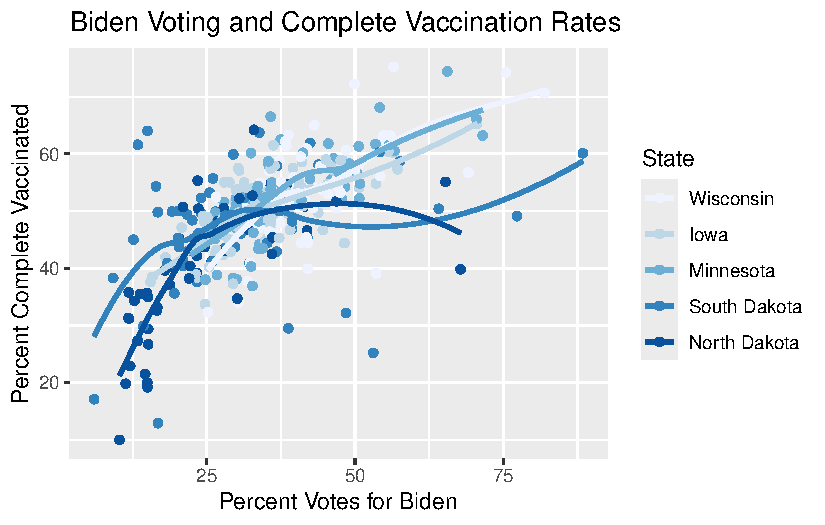
\includegraphics[keepaspectratio]{01_review164_kunsang_files/figure-pdf/unnamed-chunk-3-1.pdf}}

\begin{enumerate}
\def\labelenumi{\alph{enumi})}
\setcounter{enumi}{1}
\tightlist
\item
  One plot per state containing a scatterplot and a smoother.
\end{enumerate}

\begin{Shaded}
\begin{Highlighting}[]
\FunctionTok{library}\NormalTok{(tidyverse)}
\NormalTok{vaccine\_data }\SpecialCharTok{|\textgreater{}}
  \FunctionTok{filter}\NormalTok{(state }\SpecialCharTok{\%in\%} \FunctionTok{c}\NormalTok{(}\StringTok{"Minnesota"}\NormalTok{, }\StringTok{"Wisconsin"}\NormalTok{, }\StringTok{"Iowa"}\NormalTok{, }\StringTok{"North Dakota"}\NormalTok{, }\StringTok{"South Dakota"}\NormalTok{)) }\SpecialCharTok{|\textgreater{}}
  \FunctionTok{ggplot}\NormalTok{(}\FunctionTok{aes}\NormalTok{(}\AttributeTok{x =}\NormalTok{ perc\_Biden, }\AttributeTok{y =}\NormalTok{ perc\_complete\_vac, }\AttributeTok{color =} \FunctionTok{fct\_reorder2}\NormalTok{(state, perc\_Biden, perc\_complete\_vac))) }\SpecialCharTok{+}
  \FunctionTok{geom\_point}\NormalTok{() }\SpecialCharTok{+} \FunctionTok{geom\_smooth}\NormalTok{(}\AttributeTok{se =} \ConstantTok{FALSE}\NormalTok{) }\SpecialCharTok{+}
  \FunctionTok{labs}\NormalTok{(}
    \AttributeTok{title =} \StringTok{"Biden Voting and Complete Vaccination Rates"}\NormalTok{,}
    \AttributeTok{x =} \StringTok{"Percent Votes for Biden"}\NormalTok{,}
    \AttributeTok{y =} \StringTok{"Percent Complete Vaccinated"}\NormalTok{,}
    \AttributeTok{color =} \StringTok{"State"}
\NormalTok{  ) }\SpecialCharTok{+}
  \FunctionTok{scale\_color\_brewer}\NormalTok{() }\SpecialCharTok{+}
  \FunctionTok{facet\_wrap}\NormalTok{(}\StringTok{"state"}\NormalTok{)}
\end{Highlighting}
\end{Shaded}

\begin{verbatim}
`geom_smooth()` using method = 'loess' and formula = 'y ~ x'
\end{verbatim}

\pandocbounded{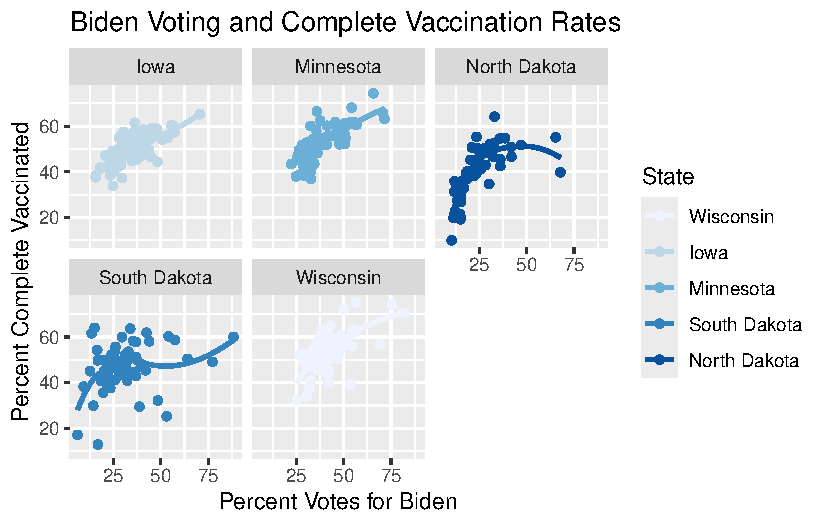
\includegraphics[keepaspectratio]{01_review164_kunsang_files/figure-pdf/unnamed-chunk-4-1.pdf}}

Describe which plot you prefer and why. What can you learn from your
preferred plot?

For overall trends, I would prefer the first plot, because it is easier
to look at how often people get vaccinated when the plots are all put
together on one graph. I can learn that Wisconsin has the highest rate
of complete vaccinations in the Midwest states we selected and that
South Dakota had the highest percentage of people who voted for Biden.

\begin{enumerate}
\def\labelenumi{\arabic{enumi}.}
\setcounter{enumi}{1}
\tightlist
\item
  We wish to compare the proportions of counties in each region with
  median household income above the national median (\$69,560).
\end{enumerate}

\begin{enumerate}
\def\labelenumi{\alph{enumi})}
\tightlist
\item
  Fill in the blanks below to produce a segmented bar plot with regions
  ordered from highest proportion above the median to lowest.
\end{enumerate}

\begin{Shaded}
\begin{Highlighting}[]
\NormalTok{vaccine\_data }\SpecialCharTok{|\textgreater{}}
  \FunctionTok{mutate}\NormalTok{(}\AttributeTok{HHincome\_vs\_national =} \FunctionTok{ifelse}\NormalTok{(median\_HHincome\_2019 }\SpecialCharTok{\textless{}} \DecValTok{69560}\NormalTok{, }\StringTok{"Less"}\NormalTok{, }\StringTok{"More"}\NormalTok{)) }\SpecialCharTok{|\textgreater{}}
  \FunctionTok{mutate}\NormalTok{(}\AttributeTok{region\_sort =} \FunctionTok{fct\_relevel}\NormalTok{(region, }\StringTok{"Northeast"}\NormalTok{, }\StringTok{"West"}\NormalTok{, }\StringTok{"South"}\NormalTok{, }\StringTok{"Midwest"}\NormalTok{)) }\SpecialCharTok{|\textgreater{}}
  \FunctionTok{ggplot}\NormalTok{(}\AttributeTok{mapping =} \FunctionTok{aes}\NormalTok{(}\AttributeTok{x =}\NormalTok{ region\_sort, }\AttributeTok{fill =}\NormalTok{ HHincome\_vs\_national)) }\SpecialCharTok{+}
    \FunctionTok{geom\_bar}\NormalTok{(}\AttributeTok{position =} \StringTok{"fill"}\NormalTok{)}
\end{Highlighting}
\end{Shaded}

\begin{enumerate}
\def\labelenumi{\alph{enumi})}
\setcounter{enumi}{1}
\tightlist
\item
  Create a table of proportions by region to illustrate that your bar
  plot in (a) is in the correct order (you should find two regions that
  are \emph{really} close when you just try to eyeball differences).
\end{enumerate}

\begin{Shaded}
\begin{Highlighting}[]
\NormalTok{newvax }\OtherTok{\textless{}{-}}\NormalTok{ vaccine\_data }\SpecialCharTok{|\textgreater{}}
  \FunctionTok{mutate}\NormalTok{(}\AttributeTok{HHincome\_vs\_national =} \FunctionTok{ifelse}\NormalTok{(median\_HHincome\_2019 }\SpecialCharTok{\textless{}} \DecValTok{69560}\NormalTok{, }\StringTok{"Less"}\NormalTok{, }\StringTok{"More"}\NormalTok{)) }\SpecialCharTok{|\textgreater{}}
  \FunctionTok{group\_by}\NormalTok{(region) }\SpecialCharTok{|\textgreater{}} 
  \FunctionTok{summarize}\NormalTok{(}\AttributeTok{income\_prop =} \FunctionTok{mean}\NormalTok{(HHincome\_vs\_national }\SpecialCharTok{==} \StringTok{"Less"}\NormalTok{))}
\NormalTok{newvax}
\end{Highlighting}
\end{Shaded}

\begin{verbatim}
# A tibble: 4 x 2
  region    income_prop
  <chr>           <dbl>
1 Midwest         0.903
2 Northeast       0.700
3 South           0.904
4 West            0.752
\end{verbatim}

\begin{enumerate}
\def\labelenumi{\alph{enumi})}
\setcounter{enumi}{2}
\tightlist
\item
  Explain why we can replace
  \texttt{fct\_relevel(region,\ FILL\ IN\ CODE)} with
\end{enumerate}

\texttt{mutate(region\_sort\ =\ fct\_reorder(region,\ median\_HHincome\_2019\ \textless{}\ 69560,\ .fun\ =\ mean))}

\begin{Shaded}
\begin{Highlighting}[]
\NormalTok{vaccine\_data }\SpecialCharTok{|\textgreater{}}
  \FunctionTok{mutate}\NormalTok{(}\AttributeTok{HHincome\_vs\_national =} \FunctionTok{ifelse}\NormalTok{(median\_HHincome\_2019 }\SpecialCharTok{\textless{}} \DecValTok{69560}\NormalTok{, }\StringTok{"Less"}\NormalTok{, }\StringTok{"More"}\NormalTok{)) }\SpecialCharTok{|\textgreater{}}
\FunctionTok{mutate}\NormalTok{(}\AttributeTok{region\_sort =} \FunctionTok{fct\_reorder}\NormalTok{(region, median\_HHincome\_2019 }\SpecialCharTok{\textless{}} \DecValTok{69560}\NormalTok{, }\AttributeTok{.fun =}\NormalTok{ mean)) }\SpecialCharTok{|\textgreater{}}
  \FunctionTok{ggplot}\NormalTok{(}\AttributeTok{mapping =} \FunctionTok{aes}\NormalTok{(}\AttributeTok{x =}\NormalTok{ region\_sort, }\AttributeTok{fill =}\NormalTok{ HHincome\_vs\_national)) }\SpecialCharTok{+}
    \FunctionTok{geom\_bar}\NormalTok{(}\AttributeTok{position =} \StringTok{"fill"}\NormalTok{)}
\end{Highlighting}
\end{Shaded}

\pandocbounded{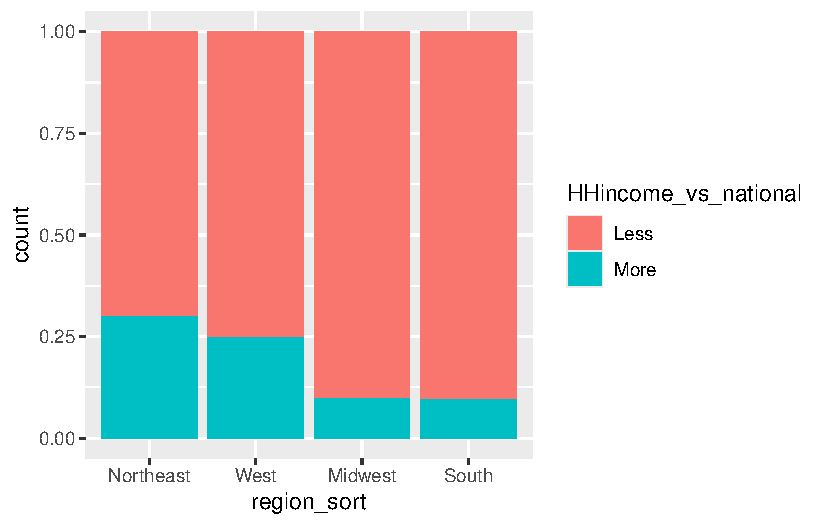
\includegraphics[keepaspectratio]{01_review164_kunsang_files/figure-pdf/unnamed-chunk-7-1.pdf}}

but not

\texttt{mutate(region\_sort\ =\ fct\_reorder(region,\ median\_HHincome\_2019\ \textless{}\ 69560))}

\begin{Shaded}
\begin{Highlighting}[]
\NormalTok{vaccine\_data }\SpecialCharTok{|\textgreater{}}
  \FunctionTok{mutate}\NormalTok{(}\AttributeTok{HHincome\_vs\_national =} \FunctionTok{ifelse}\NormalTok{(median\_HHincome\_2019 }\SpecialCharTok{\textless{}} \DecValTok{69560}\NormalTok{, }\StringTok{"Less"}\NormalTok{, }\StringTok{"More"}\NormalTok{)) }\SpecialCharTok{|\textgreater{}}
\FunctionTok{mutate}\NormalTok{(}\AttributeTok{region\_sort =} \FunctionTok{fct\_reorder}\NormalTok{(region, median\_HHincome\_2019 }\SpecialCharTok{\textless{}} \DecValTok{69560}\NormalTok{)) }\SpecialCharTok{|\textgreater{}}
  \FunctionTok{ggplot}\NormalTok{(}\AttributeTok{mapping =} \FunctionTok{aes}\NormalTok{(}\AttributeTok{x =}\NormalTok{ region\_sort, }\AttributeTok{fill =}\NormalTok{ HHincome\_vs\_national)) }\SpecialCharTok{+}
    \FunctionTok{geom\_bar}\NormalTok{(}\AttributeTok{position =} \StringTok{"fill"}\NormalTok{)}
\end{Highlighting}
\end{Shaded}

\pandocbounded{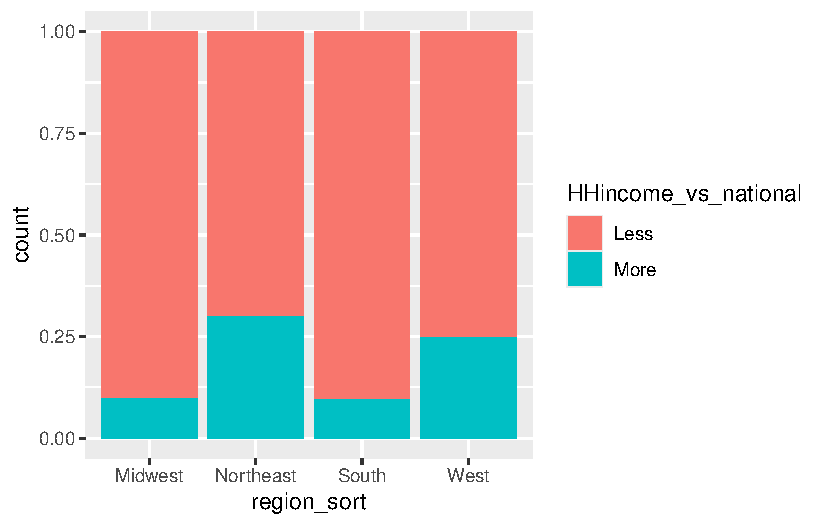
\includegraphics[keepaspectratio]{01_review164_kunsang_files/figure-pdf/unnamed-chunk-8-1.pdf}}

You can't replace the code without .fun because then there is no value
for R to compare the differing incomes to. The .fun provides a summary
statistic in the form of the mean that can then be placed in order.

\begin{Shaded}
\begin{Highlighting}[]
\CommentTok{\# og code}

\StringTok{\textquotesingle{}}
\StringTok{vaccine\_data |\textgreater{}}
\StringTok{  mutate(HHincome\_vs\_national = ifelse(median\_HHincome\_2019 \textless{} 69560, FILL IN CODE)) |\textgreater{}}
\StringTok{  mutate(region\_sort = fct\_relevel(region, FILL IN CODE)) |\textgreater{}}
\StringTok{  ggplot(mapping = aes(x = region\_sort, fill = HHincome\_vs\_national)) +}
\StringTok{    geom\_bar(position = "fill") \textquotesingle{}}
\end{Highlighting}
\end{Shaded}

\begin{enumerate}
\def\labelenumi{\arabic{enumi}.}
\setcounter{enumi}{2}
\tightlist
\item
  We want to examine the distribution of total county populations and
  then see how it's related to vaccination rates.
\end{enumerate}

\begin{enumerate}
\def\labelenumi{\alph{enumi})}
\tightlist
\item
  \emph{Carefully and thoroughly} explain why the two histograms below
  provide different plots.
\end{enumerate}

\begin{Shaded}
\begin{Highlighting}[]
\NormalTok{vaccine\_data }\SpecialCharTok{|\textgreater{}}
  \FunctionTok{mutate}\NormalTok{(}\AttributeTok{tot\_pop\_millions =}\NormalTok{ tot\_pop }\SpecialCharTok{/} \DecValTok{1000000}\NormalTok{) }\SpecialCharTok{|\textgreater{}}
  \FunctionTok{ggplot}\NormalTok{(}\AttributeTok{mapping =} \FunctionTok{aes}\NormalTok{(}\AttributeTok{x =}\NormalTok{ tot\_pop\_millions)) }\SpecialCharTok{+}
    \FunctionTok{geom\_histogram}\NormalTok{(}\AttributeTok{bins =} \DecValTok{40}\NormalTok{) }\SpecialCharTok{+}
    \FunctionTok{labs}\NormalTok{(}\AttributeTok{x =} \StringTok{"Total population in millions"}\NormalTok{)}
\end{Highlighting}
\end{Shaded}

\pandocbounded{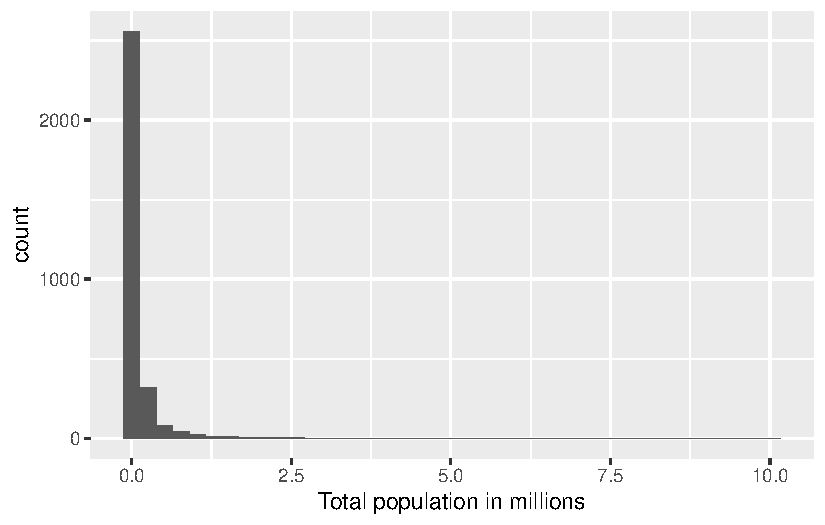
\includegraphics[keepaspectratio]{01_review164_kunsang_files/figure-pdf/unnamed-chunk-10-1.pdf}}

\begin{Shaded}
\begin{Highlighting}[]
\NormalTok{vaccine\_data }\SpecialCharTok{|\textgreater{}}
  \FunctionTok{mutate}\NormalTok{(}\AttributeTok{tot\_pop\_millions =}\NormalTok{ tot\_pop }\SpecialCharTok{\%/\%} \DecValTok{1000000}\NormalTok{) }\SpecialCharTok{|\textgreater{}}
  \FunctionTok{ggplot}\NormalTok{(}\AttributeTok{mapping =} \FunctionTok{aes}\NormalTok{(}\AttributeTok{x =}\NormalTok{ tot\_pop\_millions)) }\SpecialCharTok{+}
    \FunctionTok{geom\_histogram}\NormalTok{(}\AttributeTok{bins =} \DecValTok{40}\NormalTok{) }\SpecialCharTok{+}
    \FunctionTok{labs}\NormalTok{(}\AttributeTok{x =} \StringTok{"Total population in millions"}\NormalTok{)}
\end{Highlighting}
\end{Shaded}

\pandocbounded{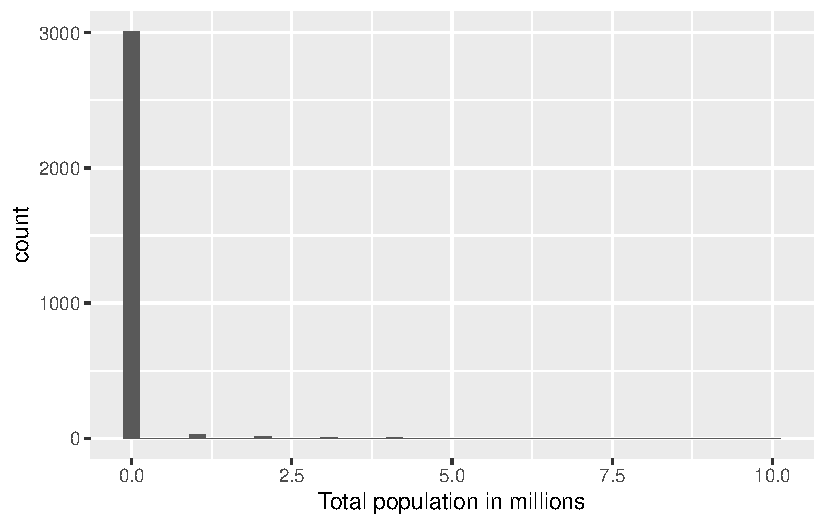
\includegraphics[keepaspectratio]{01_review164_kunsang_files/figure-pdf/unnamed-chunk-10-2.pdf}}

\begin{enumerate}
\def\labelenumi{\alph{enumi})}
\setcounter{enumi}{1}
\item
  Find the top 5 counties in terms of total population.
\item
  Plot a histogram of logged population and describe this distribution.
\item
  Plot the relationship between log population and percent vaccinated
  using separate colors for Metro and Non-metro counties (be sure
  there's no 3rd color used for NAs). Reduce the size and transparency
  of each point to make the plot more readable. Describe what you can
  learn from this plot.
\end{enumerate}

\begin{enumerate}
\def\labelenumi{\arabic{enumi}.}
\setcounter{enumi}{3}
\tightlist
\item
  Produce 3 different plots for illustrating the relationship between
  the rural\_urban\_code and percent vaccinated.
\end{enumerate}

Hint: you can sometimes turn numeric variables into categorical
variables for plotting purposes (e.g.~\texttt{as.factor()},
\texttt{ifelse()}).

\begin{Shaded}
\begin{Highlighting}[]
\NormalTok{vaccine\_data }\SpecialCharTok{|\textgreater{}} 
   \FunctionTok{ggplot}\NormalTok{(}\AttributeTok{mapping =} \FunctionTok{aes}\NormalTok{(}\AttributeTok{x =} \FunctionTok{as.factor}\NormalTok{(rural\_urban\_code), }
                        \AttributeTok{y =}\NormalTok{ perc\_complete\_vac)) }\SpecialCharTok{+}
  \FunctionTok{geom\_boxplot}\NormalTok{()}
\end{Highlighting}
\end{Shaded}

\pandocbounded{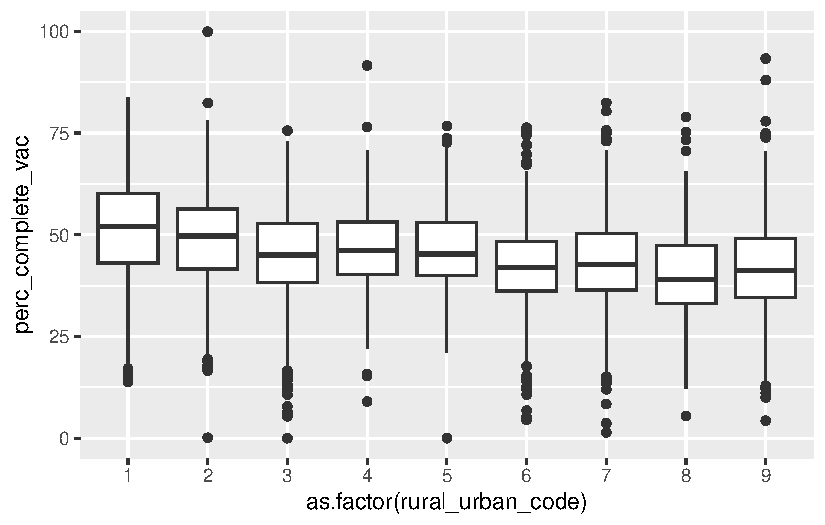
\includegraphics[keepaspectratio]{01_review164_kunsang_files/figure-pdf/unnamed-chunk-11-1.pdf}}

\begin{Shaded}
\begin{Highlighting}[]
\NormalTok{vaccine\_data }\SpecialCharTok{|\textgreater{}} 
   \FunctionTok{ggplot}\NormalTok{(}\AttributeTok{mapping =} \FunctionTok{aes}\NormalTok{(}\AttributeTok{x =} \FunctionTok{as.factor}\NormalTok{(rural\_urban\_code),}
                        \AttributeTok{fill =}\NormalTok{ perc\_complete\_vac }\SpecialCharTok{\textgreater{}} \DecValTok{50}\NormalTok{)) }\SpecialCharTok{+}
            \FunctionTok{geom\_bar}\NormalTok{(}\AttributeTok{position =} \StringTok{"fill"}\NormalTok{) }\SpecialCharTok{+}
  \FunctionTok{labs}\NormalTok{(}\AttributeTok{x =} \StringTok{"Urban to Rural Scale"}\NormalTok{,}
       \AttributeTok{y =} \StringTok{"Proportion of Complete Vaccinations over 50\%"}\NormalTok{,}
       \AttributeTok{fill =} \StringTok{"Complete Vaccinations over 50\%"}\NormalTok{,}
       \AttributeTok{title =} \StringTok{"Urban to Rural Regions and the Proportion of Complete Vaccinations"}\NormalTok{)}
\end{Highlighting}
\end{Shaded}

\pandocbounded{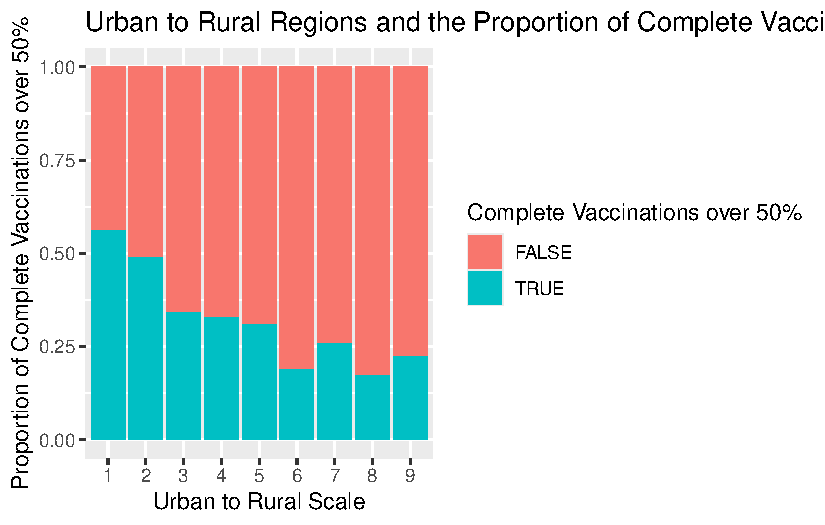
\includegraphics[keepaspectratio]{01_review164_kunsang_files/figure-pdf/unnamed-chunk-12-1.pdf}}

\begin{Shaded}
\begin{Highlighting}[]
\NormalTok{vaccine\_data }\SpecialCharTok{|\textgreater{}} 
   \FunctionTok{ggplot}\NormalTok{(}\AttributeTok{mapping =} \FunctionTok{aes}\NormalTok{(}\AttributeTok{x =}\NormalTok{ rural\_urban\_code,}
                        \AttributeTok{y =}\NormalTok{ perc\_complete\_vac)) }\SpecialCharTok{+}
  \FunctionTok{geom\_point}\NormalTok{() }\SpecialCharTok{+} 
  \FunctionTok{geom\_smooth}\NormalTok{(}\AttributeTok{method =} \StringTok{"lm"}\NormalTok{)}
\end{Highlighting}
\end{Shaded}

\begin{verbatim}
`geom_smooth()` using formula = 'y ~ x'
\end{verbatim}

\pandocbounded{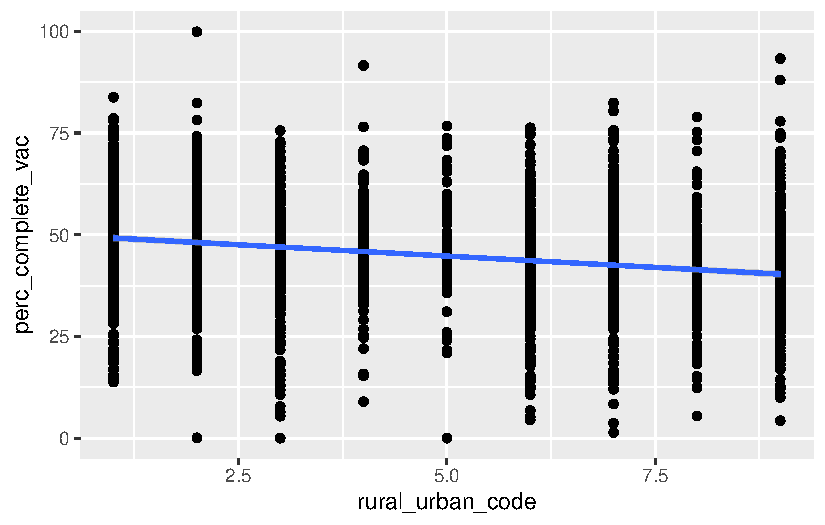
\includegraphics[keepaspectratio]{01_review164_kunsang_files/figure-pdf/unnamed-chunk-13-1.pdf}}

State your favorite plot, why you like it better than the other two, and
what you can learn from your favorite plot. Create an alt text
description of your favorite plot, using the Four Ingredient Model. See
\href{https://drive.google.com/file/d/1BuEbL6vETBcFULmtlrwwZBUYhdEg0Zqb/view?usp=sharing}{this
link} for reminders and references about alt text.

My favorite plot was the segmented bar chart because I felt it was
personally the most readable of the graphs. I can see the county with
the least complete vaccinations.

This is a segmented bar graph showing the proportion of regions with at
least 50\% complete vaccinations and ordered based on how rural and
urban they are. The X axis is measured on the urban to rural scale, a
discrete range going from 1 to 9, with 1 being the most urban region,
and 9 being the most rural region. The Y axis displays the proportion of
complete vaccinations over 50\%, where the proportions range from 0 to 1
and goes up in intervals of 0.25. The graph is segmented by two colors
showing that a given urban to rural area on the X axis had a certain
proportion of complete vaccinations that it is scaled to on the Y axis.
From the graph, the most urban regions had the highest proportion of
regions with vaccinations over 50\%, at around 58\%. The rest of the
graph shows an overall trend of decreased vaccination rates the higher
the regions scored on the urban to rural scale, with the regions on the
eighth section reaching the lowest of around 20\% having at least half
of the population vaccinated.

\begin{enumerate}
\def\labelenumi{\arabic{enumi}.}
\setcounter{enumi}{4}
\tightlist
\item
  BEFORE running the code below, sketch the plot that will be produced
  by R. AFTER running the code, describe what conclusion(s) can we draw
  from this plot?
\end{enumerate}

\begin{Shaded}
\begin{Highlighting}[]
\NormalTok{vaccine\_data }\SpecialCharTok{|\textgreater{}}
  \FunctionTok{filter}\NormalTok{(}\SpecialCharTok{!}\FunctionTok{is.na}\NormalTok{(perc\_Biden)) }\SpecialCharTok{|\textgreater{}}
  \FunctionTok{mutate}\NormalTok{(}\AttributeTok{big\_states =} \FunctionTok{fct\_lump}\NormalTok{(state, }\AttributeTok{n =} \DecValTok{10}\NormalTok{)) }\SpecialCharTok{|\textgreater{}}
  \FunctionTok{group\_by}\NormalTok{(big\_states) }\SpecialCharTok{|\textgreater{}}
  \FunctionTok{summarize}\NormalTok{(}\AttributeTok{IQR\_Biden =} \FunctionTok{IQR}\NormalTok{(perc\_Biden)) }\SpecialCharTok{|\textgreater{}}
  \FunctionTok{mutate}\NormalTok{(}\AttributeTok{big\_states =} \FunctionTok{fct\_reorder}\NormalTok{(big\_states, IQR\_Biden)) }\SpecialCharTok{|\textgreater{}}
  \FunctionTok{ggplot}\NormalTok{() }\SpecialCharTok{+} 
    \FunctionTok{geom\_point}\NormalTok{(}\FunctionTok{aes}\NormalTok{(}\AttributeTok{x =}\NormalTok{ IQR\_Biden, }\AttributeTok{y =}\NormalTok{ big\_states))}
\end{Highlighting}
\end{Shaded}

Virginia has the biggest range in Biden voters. Tennessee is more
homogeneous with its voting trends. Graphing the IQR is something new to
me, it's a good way to quantify ranges.

\begin{enumerate}
\def\labelenumi{\arabic{enumi}.}
\setcounter{enumi}{5}
\tightlist
\item
  In this question we will focus only on the 12 states in the Midwest
  (i.e.~where region == ``Midwest'').
\end{enumerate}

\begin{enumerate}
\def\labelenumi{\alph{enumi})}
\tightlist
\item
  Create a tibble with the following information for each state. Order
  states from least to greatest state population.
\end{enumerate}

\begin{itemize}
\tightlist
\item
  number of different \texttt{rural\_urban\_code}s represented among the
  state's counties (there are 9 possible)
\item
  total state population
\item
  proportion of Metro counties
\item
  median unemployment rate
\end{itemize}

\begin{Shaded}
\begin{Highlighting}[]
\NormalTok{midwest\_data }\OtherTok{\textless{}{-}}\NormalTok{ vaccine\_data }\SpecialCharTok{|\textgreater{}}
  \FunctionTok{filter}\NormalTok{(region }\SpecialCharTok{==} \StringTok{"Midwest"}\NormalTok{) }\SpecialCharTok{|\textgreater{}}
  \FunctionTok{group\_by}\NormalTok{(state) }\SpecialCharTok{|\textgreater{}}
  \FunctionTok{summarize}\NormalTok{(}\AttributeTok{uniquecode =} \FunctionTok{n\_distinct}\NormalTok{(rural\_urban\_code),}
            \AttributeTok{tot\_state\_pop =} \FunctionTok{sum}\NormalTok{(tot\_pop),}
            \AttributeTok{prop\_metro =} \FunctionTok{mean}\NormalTok{(metro\_status }\SpecialCharTok{==} \StringTok{"Metro"}\NormalTok{), }
            \AttributeTok{median\_unemp =} \FunctionTok{median}\NormalTok{(unemployment\_rate\_2020)) }\SpecialCharTok{|\textgreater{}}
  \FunctionTok{arrange}\NormalTok{(}\FunctionTok{desc}\NormalTok{(tot\_state\_pop))}
\NormalTok{midwest\_data}
\end{Highlighting}
\end{Shaded}

\begin{verbatim}
# A tibble: 12 x 5
   state        uniquecode tot_state_pop prop_metro median_unemp
   <chr>             <int>         <dbl>      <dbl>        <dbl>
 1 Illinois              9      12671821      0.392         7.75
 2 Ohio                  7      11689100      0.432         8.1 
 3 Michigan              9       9986857      0.313         9.1 
 4 Indiana               8       6732219      0.478         6.5 
 5 Missouri              9       6137428      0.296         5.6 
 6 Wisconsin             8       5822434      0.361         6.3 
 7 Minnesota             9       5639632      0.310         5.6 
 8 Iowa                  8       3155070      0.212         4.6 
 9 Kansas                9       2913314      0.181         4.1 
10 Nebraska              6       1261262      0.292         3.3 
11 South Dakota          6        884659      0.121         4.35
12 North Dakota          6        762062      0.113         4.4 
\end{verbatim}

\begin{enumerate}
\def\labelenumi{\alph{enumi})}
\setcounter{enumi}{1}
\tightlist
\item
  Use your tibble in (a) to produce a plot of the relationship between
  proportion of Metro counties and median unemployment rate. Points
  should be colored by the number of different
  \texttt{rural\_urban\_code}s in a state, but a single linear trend
  should be fit to all points. What can you conclude from the plot?
\end{enumerate}

\begin{Shaded}
\begin{Highlighting}[]
\NormalTok{midwest\_data }\SpecialCharTok{|\textgreater{}} 
  \FunctionTok{ggplot}\NormalTok{(}\FunctionTok{aes}\NormalTok{(}\AttributeTok{x =}\NormalTok{ prop\_metro,}
             \AttributeTok{y =}\NormalTok{ median\_unemp,}
             \AttributeTok{color =}\NormalTok{ uniquecode)) }\SpecialCharTok{+}
  \FunctionTok{geom\_point}\NormalTok{() }\SpecialCharTok{+} \FunctionTok{geom\_smooth}\NormalTok{(}\AttributeTok{method =} \StringTok{"lm"}\NormalTok{, }\AttributeTok{se =} \ConstantTok{FALSE}\NormalTok{)}
\end{Highlighting}
\end{Shaded}

\begin{verbatim}
`geom_smooth()` using formula = 'y ~ x'
\end{verbatim}

\begin{verbatim}
Warning: The following aesthetics were dropped during statistical transformation:
colour.
i This can happen when ggplot fails to infer the correct grouping structure in
  the data.
i Did you forget to specify a `group` aesthetic or to convert a numerical
  variable into a factor?
\end{verbatim}

\pandocbounded{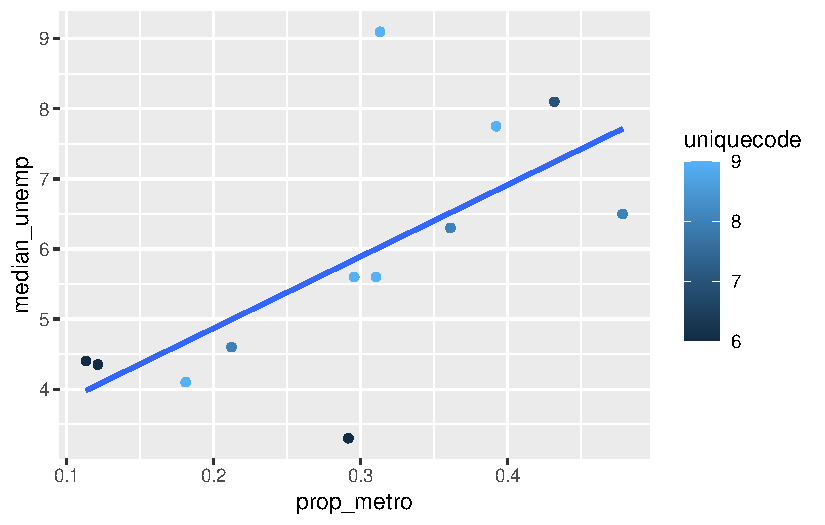
\includegraphics[keepaspectratio]{01_review164_kunsang_files/figure-pdf/unnamed-chunk-16-1.pdf}}

From the plot I can conclude that the higher the proportion of counties
that are metro, on average the median unemployment rate rises as well.

\begin{enumerate}
\def\labelenumi{\arabic{enumi}.}
\setcounter{enumi}{6}
\tightlist
\item
  Generate an appropriate plot to compare vaccination rates between two
  subregions of the US: New England (which contains the states Maine,
  Vermont, New Hampshire, Massachusetts, Connecticut, Rhode Island) and
  the Upper Midwest (which, according to the USGS, contains the states
  Minnesota, Wisconsin, Michigan, Illinois, Indiana, and Iowa). What can
  you conclude from your plot?
\end{enumerate}

\begin{Shaded}
\begin{Highlighting}[]
\CommentTok{\#do this later}
\end{Highlighting}
\end{Shaded}

In this next section, we consider a few variables that could have been
included in our data set, but were NOT. Thus, you won't be able to write
and test code, but you nevertheless should be able to use your knowledge
of the tidyverse to answer these questions.

Here are the hypothetical variables:

\begin{itemize}
\tightlist
\item
  HR\_party = party of that county's US Representative (Republican,
  Democrat, Independent, Green, or Libertarian)
\item
  people\_per\_MD = number of residents per doctor (higher values =
  fewer doctors)
\item
  perc\_over\_65 = percent of residents over 65 years old
\item
  perc\_white = percent of residents who identify as white
\end{itemize}

\begin{enumerate}
\def\labelenumi{\arabic{enumi}.}
\setcounter{enumi}{7}
\tightlist
\item
  Hypothetical R chunk \#1:
\end{enumerate}

\begin{Shaded}
\begin{Highlighting}[]
\CommentTok{\# Hypothetical R chunk 1}
\NormalTok{temp }\OtherTok{\textless{}{-}}\NormalTok{ vaccine\_data }\SpecialCharTok{|\textgreater{}}
  \FunctionTok{mutate}\NormalTok{(}\AttributeTok{new\_perc\_vac =} \FunctionTok{ifelse}\NormalTok{(perc\_complete\_vac }\SpecialCharTok{\textgreater{}} \DecValTok{95}\NormalTok{, }\ConstantTok{NA}\NormalTok{, perc\_complete\_vac),}
         \AttributeTok{MD\_group =} \FunctionTok{cut\_number}\NormalTok{(people\_per\_MD, }\DecValTok{3}\NormalTok{)) }\SpecialCharTok{|\textgreater{}}
  \FunctionTok{group\_by}\NormalTok{(MD\_group) }\SpecialCharTok{|\textgreater{}}
  \FunctionTok{summarise}\NormalTok{(}\AttributeTok{n =} \FunctionTok{n}\NormalTok{(),}
            \AttributeTok{mean\_perc\_vac =} \FunctionTok{mean}\NormalTok{(new\_perc\_vac, }\AttributeTok{na.rm =} \ConstantTok{TRUE}\NormalTok{),}
            \AttributeTok{mean\_white =} \FunctionTok{mean}\NormalTok{(perc\_white, }\AttributeTok{na.rm =} \ConstantTok{TRUE}\NormalTok{))}
\end{Highlighting}
\end{Shaded}

\begin{enumerate}
\def\labelenumi{\alph{enumi})}
\tightlist
\item
  Describe the tibble \texttt{temp} created above. What would be the
  dimensions? What do rows and columns represent?
\end{enumerate}

Group\_by tells us how many rows are in the tibble which is 3 because 3
groups were made by the cut\_number function, the numbers of columns are
given by the summarize function (at least 3), and then 1 more for the
group name. This temp tibble is 3 rows by 4 columns. Each row represents
one third of the data when it has been altered by the cut\_number
function, and then the summarized data from within the first third of
the data has had the count of observations, mean of the percent
vaccinated, and the mean of the percentage of white population.

\begin{enumerate}
\def\labelenumi{\alph{enumi})}
\setcounter{enumi}{1}
\tightlist
\item
  What would happen if we replaced
  \texttt{new\_perc\_vac\ =\ ifelse(perc\_complete\_vac\ \textgreater{}\ 95,\ NA,\ perc\_complete\_vac)}
  with
  \texttt{new\_perc\_vac\ =\ ifelse(perc\_complete\_vac\ \textgreater{}\ 95,\ perc\_complete\_vac,\ NA)}?
\end{enumerate}

If we switched the orders then the percentages that are over 95 get set
to perc\_complete\_vac as opposed to NA values and the ones that are
under or equal to 95 get set to NA. The remaining values are then
switched to be much higher when the mean is taken of new\_perc\_vac,
with all the NA values being removed.

\begin{enumerate}
\def\labelenumi{\alph{enumi})}
\setcounter{enumi}{2}
\tightlist
\item
  What would happen if we replaced
  \texttt{mean\_white\ =\ mean(perc\_white,\ na.rm\ =\ TRUE)} with
  \texttt{mean\_white\ =\ mean(perc\_white)}?
\end{enumerate}

If we removed the na.rm = TRUE then the NA values would remain and all
the values in that column would be NA, as R throws an NA value when
attempting to calculate the mean with an NA value still included.

\begin{enumerate}
\def\labelenumi{\alph{enumi})}
\setcounter{enumi}{3}
\tightlist
\item
  What would happen if we removed \texttt{group\_by(MD\_group)}?
\end{enumerate}

If we removed group\_by(MD\_group) then there would be a lot more rows
in the tibble because the group\_by function is what reduces it to only
being 3. The rest of the data set would still be there.

\begin{enumerate}
\def\labelenumi{\arabic{enumi}.}
\setcounter{enumi}{8}
\tightlist
\item
  Hypothetical R chunk \#2:
\end{enumerate}

\begin{Shaded}
\begin{Highlighting}[]
\CommentTok{\# Hypothetical R chunk 2}
\FunctionTok{ggplot}\NormalTok{(}\AttributeTok{data =}\NormalTok{ vaccine\_data) }\SpecialCharTok{+}
  \FunctionTok{geom\_point}\NormalTok{(}\AttributeTok{mapping =} \FunctionTok{aes}\NormalTok{(}\AttributeTok{x =}\NormalTok{ perc\_over\_65, }\AttributeTok{y =}\NormalTok{ perc\_complete\_vac, }
                           \AttributeTok{color =}\NormalTok{ HR\_party)) }\SpecialCharTok{+}
  \FunctionTok{geom\_smooth}\NormalTok{()}

\NormalTok{temp }\OtherTok{\textless{}{-}}\NormalTok{ vaccine\_data }\SpecialCharTok{|\textgreater{}}
  \FunctionTok{group\_by}\NormalTok{(HR\_party) }\SpecialCharTok{|\textgreater{}}
  \FunctionTok{summarise}\NormalTok{(}\AttributeTok{var1 =} \FunctionTok{n}\NormalTok{()) }\SpecialCharTok{|\textgreater{}}
  \FunctionTok{arrange}\NormalTok{(}\FunctionTok{desc}\NormalTok{(var1)) }\SpecialCharTok{|\textgreater{}}
  \FunctionTok{slice\_head}\NormalTok{(}\AttributeTok{n =} \DecValTok{3}\NormalTok{)}

\NormalTok{vaccine\_data }\SpecialCharTok{|\textgreater{}}
  \FunctionTok{ggplot}\NormalTok{(}\AttributeTok{mapping =} \FunctionTok{aes}\NormalTok{(}\AttributeTok{x =} \FunctionTok{fct\_reorder}\NormalTok{(HR\_party, perc\_over\_65, }\AttributeTok{.fun =}\NormalTok{ median), }
                       \AttributeTok{y =}\NormalTok{ perc\_over\_65)) }\SpecialCharTok{+}
    \FunctionTok{geom\_boxplot}\NormalTok{()}
\end{Highlighting}
\end{Shaded}

\begin{enumerate}
\def\labelenumi{\alph{enumi})}
\tightlist
\item
  Why would the first plot produce an error?
\end{enumerate}

The aesthetics mapping is only sent to the geom\_point function, when it
should have been either copied into the geom\_smooth again or just put
in the ggplot to begin with. Geom\_smooth only has the data to read.

\begin{enumerate}
\def\labelenumi{\alph{enumi})}
\setcounter{enumi}{1}
\tightlist
\item
  Describe the tibble \texttt{temp} created above. What would be the
  dimensions? What do rows and columns represent?
\end{enumerate}

Arranged the rows by count of how many people align with each party in
descending order. Then the first 3 rows of people has been selected, so
there are 3 rows. There are 2 columns, one for var1 and one for the
HR\_party. (3 by 2 tibble.) The first row has the most number of people
in the political party, the second has the second most, and the third
has the third most.

\begin{enumerate}
\def\labelenumi{\alph{enumi})}
\setcounter{enumi}{2}
\tightlist
\item
  What would happen if we replaced
  \texttt{fct\_reorder(HR\_party,\ perc\_over\_65,\ .fun\ =\ median)}
  with \texttt{HR\_party}?
\end{enumerate}

The data would stay at its default status and wouldn't be leveled in
order of ascending percentages over 65.

\begin{enumerate}
\def\labelenumi{\arabic{enumi}.}
\setcounter{enumi}{9}
\tightlist
\item
  Hypothetical R chunk \#3:
\end{enumerate}

\begin{Shaded}
\begin{Highlighting}[]
\CommentTok{\# Hypothetical R chunk 3}
\NormalTok{vaccine\_data }\SpecialCharTok{|\textgreater{}}
  \FunctionTok{filter}\NormalTok{(}\SpecialCharTok{!}\FunctionTok{is.na}\NormalTok{(people\_per\_MD)) }\SpecialCharTok{|\textgreater{}}
  \FunctionTok{mutate}\NormalTok{(}\AttributeTok{state\_lump =} \FunctionTok{fct\_lump}\NormalTok{(state, }\AttributeTok{n =} \DecValTok{4}\NormalTok{)) }\SpecialCharTok{|\textgreater{}}
  \FunctionTok{group\_by}\NormalTok{(state\_lump, rural\_urban\_code) }\SpecialCharTok{|\textgreater{}}
  \FunctionTok{summarise}\NormalTok{(}\AttributeTok{mean\_people\_per\_MD =} \FunctionTok{mean}\NormalTok{(people\_per\_MD)) }\SpecialCharTok{|\textgreater{}}
  
  \FunctionTok{ggplot}\NormalTok{(}\AttributeTok{mapping =} \FunctionTok{aes}\NormalTok{(}\AttributeTok{x =}\NormalTok{ rural\_urban\_code, }\AttributeTok{y =}\NormalTok{ mean\_people\_per\_MD, }
      \AttributeTok{colour =} \FunctionTok{fct\_reorder2}\NormalTok{(state\_lump, rural\_urban\_code, mean\_people\_per\_MD))) }\SpecialCharTok{+}
    \FunctionTok{geom\_line}\NormalTok{()}
\end{Highlighting}
\end{Shaded}

\begin{enumerate}
\def\labelenumi{\alph{enumi})}
\tightlist
\item
  Describe the tibble piped into the ggplot above. What would be the
  dimensions? What do rows and columns represent?
\end{enumerate}

Five rows created by the fct\_lump. The four most common states have
been preserved, with the rest being put into an other category. They are
then grouped by state and how rural and urban they are, which adds on 2
columns as well as one more column for the mean\_people\_per\_MD created
by the summarize function. There are 5 rows and 3 columns.

\begin{enumerate}
\def\labelenumi{\alph{enumi})}
\setcounter{enumi}{1}
\tightlist
\item
  Carefully describe the plot created above.
\end{enumerate}

The plot created is a line graph with data points being mapped on the x
axis by the Urban to Rural scale, which goes from 1-9 (1 being the most
urban, 9 being the most rural), and on the y axis it is ranked by the
mean number of people per medical doctor. There would be 9 points made
for each line, and 5 lines made total, because the urban rural scale
groups together the data by how rural and urban the region is, and the
state\_lump function has kept 4 of the most common states with the fifth
being the remaining states grouped together. Each line will be colored
by state and then the lines will be ordered by the largest mean people
per doctor associated with the highest rural urban code, letting the
colors match the legend.

\begin{enumerate}
\def\labelenumi{\alph{enumi})}
\setcounter{enumi}{2}
\tightlist
\item
  What would happen if we removed
  \texttt{filter(!is.na(people\_per\_MD))}?
\end{enumerate}

If we removed the filter, then the mean\_people\_per\_MD would appear as
an NA value because there would be an NA value that R can't do
operations with. The ggplot would not be able to be plotted because of
the NA value.

\begin{enumerate}
\def\labelenumi{\alph{enumi})}
\setcounter{enumi}{3}
\tightlist
\item
  What would happen if we replaced
  \texttt{fct\_reorder2(state\_lump,\ rural\_urban\_code,\ mean\_people\_per\_MD)}
  with \texttt{state\_lump}?
\end{enumerate}

If we removed the fct\_reorder2 and put state\_lump instead, the colors
of rural\_urban\_code and mean\_people\_per\_MD wouldn't be ordered by
the ranked values of state\_lump and would just be categorized randomly.




\end{document}
